\documentclass{article}

\usepackage{lmodern}
\usepackage[T1]{fontenc}

\usepackage[sfdefault,light]{FiraSans}
\usepackage{geometry}
\geometry{a4paper,margin=0.8in,top=0.5in,bottom=0.5in}
\pagestyle{empty}
\setcounter{secnumdepth}{0}
\usepackage{microtype}
\usepackage{graphicx}
\usepackage{fontawesome5}
\usepackage{enumitem}
\setlist[itemize]{leftmargin=*,label=\faCaretRight,itemsep=0pt}
\usepackage{xcolor}
\definecolor{background}{HTML}{0D47A1}
\usepackage[explicit]{titlesec}
\titleformat{\section}{\large\bfseries\color{white}}{}{}{\colorbox{background}{#1}}
\titleformat{\subsubsection}{\large\itshape}{}{}{#1}
\titlespacing{\subsection}{0pt}{*3}{*0.5}
\titlespacing{\subsubsection}{0pt}{*0}{*0.5}

\newcommand{\rside}[1]{\hfill \normalfont\scshape\MakeLowercase{#1}}

\usepackage[bookmarks=false,hidelinks]{hyperref}

\begin{document}

\begin{center}
  \begin{minipage}{0.45\textwidth}
    {\Huge\bfseries Pedro Paulo \\ Almeida Rodrigues} \\[0.5ex] 
  \end{minipage}\hfill
  \begin{minipage}{0.35\textwidth}
    \faPhone\ +55 (96) 99184-9667 \\ 
    \href{mailto:apedropaulo20@gmail.com}{\faEnvelope\ apedropaulo20@gmail.com} \\
    \href{https://www.linkedin.com/in/pedro-paulo-almeida-rodrigues-a788541a1}{\faLinkedin\ Pedro Paulo Almeida Rodrigues} \\
    \href{https://github.com/PedroPaulo-98}{\faGithub\ PedroPaulo-98}
  \end{minipage}
  \begin{minipage}{0.15\textwidth}
    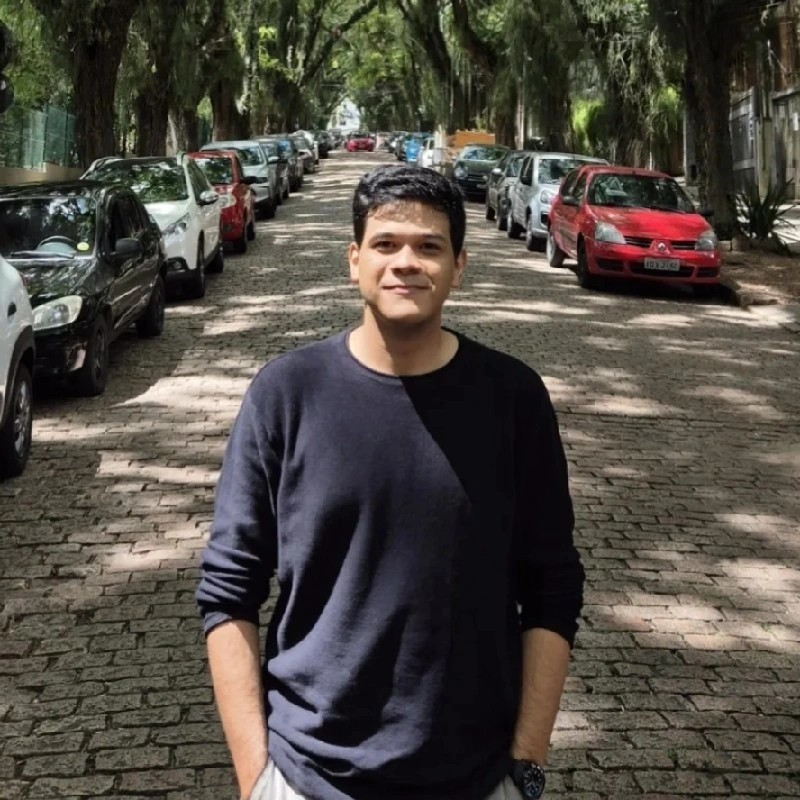
\includegraphics[width=\linewidth]{pedro.jpg}
  \end{minipage}
\end{center}

\section{\faUser\enspace About Me}
\begin{description}
  \item \ \ \ \ \ \ I am a professional passionate about technology and education. I work as a Systems Analyst at PRODAP, where I develop and provide support for governmental systems of the State of Amapá, in addition to developing systems for private companies. I have experience in software development using frameworks such as Django, Laravel, FastAPI, and others. My goal is to contribute to innovation and to improving quality of life through technology and education. \\ I am resilient, always seeking to learn and adapt quickly. I value teamwork, have a strong sense of responsibility, and am capable of performing well under pressure.
\end{description}

\section{\faCogs\enspace Skills}
\begin{description}
  \item[Traits] Hardworking, Resilient, Patient, Dedicated
  \item[Experience] PHP, Laravel, Python, FastAPI, Django, Flutter, Java, HTML, CSS, .NET, React, Ruby, Delphi, Quarkus, SQL, GIT, Docker, Portainer, BI, Dashboards, Mikrotik, and other technologies
\end{description}

\section{\faChartPie\enspace Professional Experience}

\subsection{MSB \rside{June 2025 - Present}}
\subsubsection{Full Stack Developer (working at PRODAP) \rside{Macapá, AP}}
\begin{itemize}
  \item System development (Laravel, Django, AdonisJS, React, and others)
  \item Updates and improvements to legacy systems (PHP 5 and 7, Laravel 5 and 7)
  \item Mobile development (Flutter)
  \item Data analysis (BIs and APIs)
  \item Infrastructure (Portainer, HTTPD (Apache and Nginx), and server configuration)
\end{itemize}

\subsection{TGR Studio \rside{May 2025 - September 2025}}
\subsubsection{Full Stack Developer \rside{Novo Hamburgo, RS}}
\begin{itemize}
  \item System development (Laravel)
  \item Mobile development (Flutter)
  \item E-commerce platforms
\end{itemize}

\subsection{PRODAP - Center for Information Technology Management \rside{April 2024 - June 2025}}
\subsubsection{Systems Analyst (Developer) \rside{Macapá, AP}}
\begin{itemize}
  \item Development of systems and APIs (Laravel, Django, and FastAPI)
  \item Updates and improvements to legacy systems (PHP 5 and 7, Laravel 5 and 7)
  \item Data analysis with dashboards (Looker Studio, Python, Django, and Plotly)
\end{itemize}

\subsection{PRODAP - Center for Information Technology Management \rside{June 2023 - April 2024}}
\subsubsection{Data Analyst \rside{Macapá, AP}}
\begin{itemize}
  \item Data collection and dashboard development for the State of Amapá
  \item Creation of the “Amapá Vaccinometer” (\href{http://srag.painel.prodap.ap.gov.br/vacinometro.html}{link})
  \item Government commitments tracking system
\end{itemize}

\subsection{Amapá Meta College of Technology \rside{January - June 2024}}
\subsubsection{University Professor \rside{Macapá, AP}}
\begin{itemize}
  \item Computer Architecture and Organization
  \item Computer Networks
  \item Introduction to Computer Engineering
\end{itemize}

\subsection{SESA - State Health Department of Amapá \rside{March 2023 - April 2024}}
\subsubsection{Developer and Project Management Analyst \rside{Macapá, AP}}
\begin{itemize}
  \item Development of health systems (PHP with Laravel framework)
  \item Monitoring of network infrastructure in state hospitals
  \item Creation of the SSD-AP (Amapá Digital Health System)
\end{itemize}

\subsection{IFAP – Federal Institute of Education, Science and Technology of Amapá \rside{April - June 2023}}
\subsubsection{Computer Science Instructor \rside{Mazagão, AP}}
\begin{itemize}
  \item Taught basic computing in the “Mais Cultura no Meio do Mundo” project
\end{itemize}

\subsection{Internships}
\subsubsection{Corumba Outsourcing - Support \rside{2019}}
\begin{itemize}
  \item Technical support for companies
  \item Computer maintenance
  \item Report creation for process improvements
\end{itemize}
\subsubsection{PRODAP - IT Governance \rside{November 2020 - November 2022}}
\begin{itemize}
  \item Data collection and organization for dashboards and reports
  \item Development of system usage policies
  \item Support in applying agile methodologies
\end{itemize}

\section{\faGraduationCap\enspace Education}
\subsection{Amapá Meta College of Technology \rside{January 2017 - June 2022}}
\subsubsection{Bachelor’s Degree in Computer Engineering \rside{Macapá, AP}}
\begin{itemize}
  \item \textit{Automotive Signaling Device for Hearing-Impaired Individuals}
  \item \textit{Using a Microcomputer as a Proxy Server for Small Businesses}
  \item \textit{EPI Tracking and Management System via RFID}
\end{itemize}

\subsection{Federal Institute of Education, Science and Technology of Amapá (IFAP) \rside{July 2022 - December 2023}}
\subsubsection{Postgraduate Degree in Informatics in Education \rside{Macapá, AP}}
\begin{itemize}
  \item \textit{Use of the Educ-Bio App: A biology teaching strategy for 3rd-year public high school students in Macapá}
\end{itemize}

\subsection{Pontifical Catholic University of Rio Grande do Sul (PUCRS) \rside{September 2022 - December 2023}}
\subsubsection{Postgraduate Degree in Digital Security, Governance, and Data Management \rside{Porto Alegre, RS}}
\begin{itemize}
  \item \textit{System for Monitoring and Managing Political Promises through a Dashboard Panel}
\end{itemize}

\section{\faFlask\enspace Projects}

\subsection{Amapá Jovem Registration System (2024 and 2025)}
\begin{itemize}
  \item Update of the Amapá Jovem project registration system
\end{itemize}

\subsection{Vaccinometer}
\begin{itemize}
  \item System for tracking COVID-19 cases and vaccinations in the State of Amapá (\href{http://srag.painel.prodap.ap.gov.br/vacinometro.html}{link})
\end{itemize}

\subsection{Transparency API}
\begin{itemize}
  \item API providing data on social benefits, public servants, and travel allowances (civil and military)
  \item \href{http://api.transparencia.ap.gov.br/docs}{api.transparencia.ap.gov.br/docs}
\end{itemize}

\subsection{HR System}
\begin{itemize}
  \item Internal Human Resources management system
\end{itemize}

\subsection{PROD System}
\begin{itemize}
  \item Internal documentation and infrastructure management system
\end{itemize}

\subsection{Amapá Seal System}
\begin{itemize}
  \item Certification system for regional products in the State of Amapá
\end{itemize}

\subsection{Amapá Digital Health System}
\begin{itemize}
  \item Digital system for patient intake at state hospitals
\end{itemize}

\subsection{System Development}
\begin{itemize}
  \item Systems developed using PHP, Laravel, Django, FastAPI, and others
\end{itemize}

\subsection{Legacy System Updates}
\begin{itemize}
  \item Maintenance of systems in PHP 5 and 7, Laravel 5 to 10
\end{itemize}

\href{https://github.com/PedroPaulo-98/Curriculo}{\faGithub\ Resume on GitHub}

\end{document}
